\section{Introduction}

Humans possess the remarkable ability to learn a new concept from seeing just a
few examples. A child who is learning her first few words can easily pick up
the meaning of the word ``fork" after observing only one or a handful of forks
\citep{Bloom2000}. In contrast, state-of-the-art artificial learning systems use
hundreds or thousands of examples when learning to recognize the same objects
\citep[e.g.,][]{Krizhevsky2012, Szegedy2015}. Consequently, significant
effort is ongoing to understand what neural and cognitive mechanisms enable
efficient concept learning \citep{Lake2017}. In this paper, we perform a series
of developmentally-informed neural network experiments to study the
computational basis of efficient word learning. \footnote{All experiments can be
reproduced using the code repository located at
\url{http://github.com/rfeinman/learning-to-learn}.}

\begin{figure}[h!]
    \begin{center}
        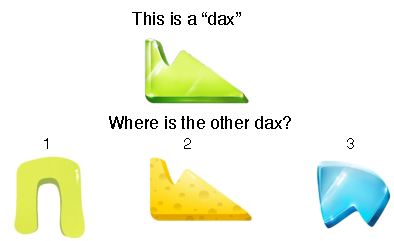
\includegraphics[width=0.3\textwidth]{figures/shape_bias_demo.pdf}
    \end{center}
    \caption{The shape bias. Children learn that objects with the same name
    tend to have the same shape, and thus option 2 above is likely the right
    answer. This inductive bias helps with future word learning.}
    \label{fig:shape_bias_demo}
\end{figure}

If humans extrapolate beyond the presented data, then another source of
information must make up the difference; prior background knowledge must
delimit the hypothesis space during learning \citep{Tenenbaum2011, Lake2017}. By
constraining the space of models considered by the learner, these priors,
referred to herein as ``inductive biases," help the learner make inferences
that go far beyond the observed data. As one manifestation, human children make
use of the shape bias--the assumption that objects that have the same name will
tend to have the same shape--when learning new object names, and thus shape is
more important than color, material and other properties when generalizing a
new label to new examples (Fig. \ref{fig:shape_bias_demo}) \citep{Landau1988}.
Similarly, children assume that object names are mutually exclusive, i.e. that
a novel name probably refers to a novel object rather than a familiar object
\citep{Markman1988}. Although the origin of inductive biases is not always
clear, results show that children, adults and primates can ``learn-to-learn" or
form higher-order generalizations that can improve the efficiency of future
learning \citep{Harlow1949, Smith2002, Dewar2010}.

Cognitive scientists have proposed a number of computational models to explain
how inductive biases are acquired and harnessed for future learning.
Hierarchical Bayesian Models (HBMs) enable probabilistic inference at multiple
levels simultaneously, allowing the model to learn the structure of individual
concepts while simultaneously learning about the structure of concepts in
general (i.e., learning a prior on new concepts)
\citep{Gelman2013, Kemp2007, Salakhutdinov2012}. These models have been used to
explain various forms of ``learning-to-learn" including learning a shape bias
\citep{Kemp2007}, yet it is currently difficult to apply HBMs to the type of
raw, high-dimensional sensory data that children receive, such as images or
audio waves. In some cases, HBMs and related approaches have been applied
successfully to raw high-dimensional data such as when learning handwritten
characters \citep{Lake2015}, but with the help of domain-specific knowledge and
engineering. In contrast, recent progress in training deep neural networks
shows how relatively generic architectures can learn effectively from raw data
\citep{LeCun2015}, providing the potential bridge between controlled simulations
with synthetic data \citep[e.g.,][]{Colunga2005} and large-scale real-world
object recognition tasks with raw data \citep[e.g.,][]{Ritter2017}. Here, we
take advantage of this connection by using neural networks to study
learning-to-learn in several different settings of varying stimulus complexity,
with the goal of isolating the fundamentals of the learning dynamics.

Most related to our work here are studies by \cite{Colunga2005} and
\cite{Ritter2017} investigating neural network accounts of shape bias
development. \cite{Colunga2005} showed that a simple neural network model,
trained via Hebbian learning, can acquire the shape bias when presented with
datasets comparable to human developmental studies. However, these simulations
operate on highly simplified bit-vector data, and it is unclear how their
results generalize to more realistic stimuli. Furthermore, the authors did not
systematically vary the structure of the training set, so we do not know the
exact conditions in which biases arise, nor whether current models are
sufficient to explain it. In a recent study, building on recent advances in
object recognition, \cite{Ritter2017} found that performance-optimized deep
neural networks (DNNs) develop the shape bias over the course of learning when
trained on the popular ImageNet classification dataset consisting of raw
naturalistic images. Although these results highlight an exciting possible
connection between DNNs and developmental psychology, many questions remain.
ImageNet--which contains thousands of labeled examples of each visual
concept--is a poor proxy for human developmental learning sets. Whether or not
these models can acquire the same bias with a training set comparable to humans
remains unknown; an answer to this question may help to explain the
developmental process in children. Furthermore, while the development of the
shape bias is known to predict the onset of vocabulary acceleration in children
\citep{GershkoffStowe2004}, we do not know whether the same holds for DNNs.

We investigate the development and influence of inductive biases in neural
network models using artificial object stimuli designed to closely mimic
developmental studies with human children. Borrowing the experimental paradigm
of \cite{Smith2002}, we evaluate the first- and second-order generalization
capabilities of neural networks trained with variable-sized datasets. Beginning
with simple bit-vector data akin to \cite{Colunga2005}, we systematically vary
the number of categories and the number of exemplars in the training set,
recording generalization performance at each pairing. Parallel experiments are
then performed with RGB image data, where each image consists of a 2D object
with a particular shape, color and texture that is shifted and placed over
white background. For each the bit-vector and RGB image data, we investigate
the parametric relationship between bias strength and attribute similarity in
our models by systematically varying the shape, color and texture attributes of
select test stimuli. Similarly, we evaluate bias strength as a function of
depth in the network. In a final set of experiments, we investigate the
correlation between shape bias acquisition and the rate of concept learning in
our networks, mirroring an analogous study from human developmental psychology
\citep{GershkoffStowe2004}.



